\section[Création Projet Laravel]{Création Projet Laravel 
\includegraphics[height=20pt]{figures-logos/laravel.pdf}}

\begin{enumerate}
    \item Si vous souhaitez créer un nouveau projet vierge, allez à la \textsc{section~\ref{sec:new_project}}.
    \item Si vous souhaitez importer un projet depuis \github{}, allez à la \textsc{section~\ref{sec:project_git}}.
\end{enumerate}

\subsection[Création d'un nouveau projet]{Création d'un nouveau projet\label{sec:new_project}}
    \subsubsection[Création du dossier]{Création du dossier}
        Pour créer un nouveau projet \laravel{} dans un dossier ``exemple-app'' il suffit juste d'entrer la ligne de commande:

        \begin{lstlisting}
            curl -s https://laravel.build/example-app | bash
        \end{lstlisting}

        Avec cette commande votre projet sera installé avec plusieurs services de base (mysql, redis, et d'autres). PS:la création peut prendre du temps (5\-10 minutes).

        il est possible de choisir les services à installer avec le mot clé \textit{with}. Dans le cadre de ce tutoriel, nous aurons besoin de 3 services: \mysql, mailpit et \phpmyadmin. Les 2 premiers peuvent être téléchargés avec laravel comme suit:

        \begin{lstlisting}
            curl -s "https://laravel.build/example-app?with=mysql,mailpit" | bash
        \end{lstlisting}

        une fois la commande lancée le projet va se créer (cela peut prendre un certain temps)

        \begin{figure}[h]
            \centering
            \begin{subfigure}{0.3\textwidth}
                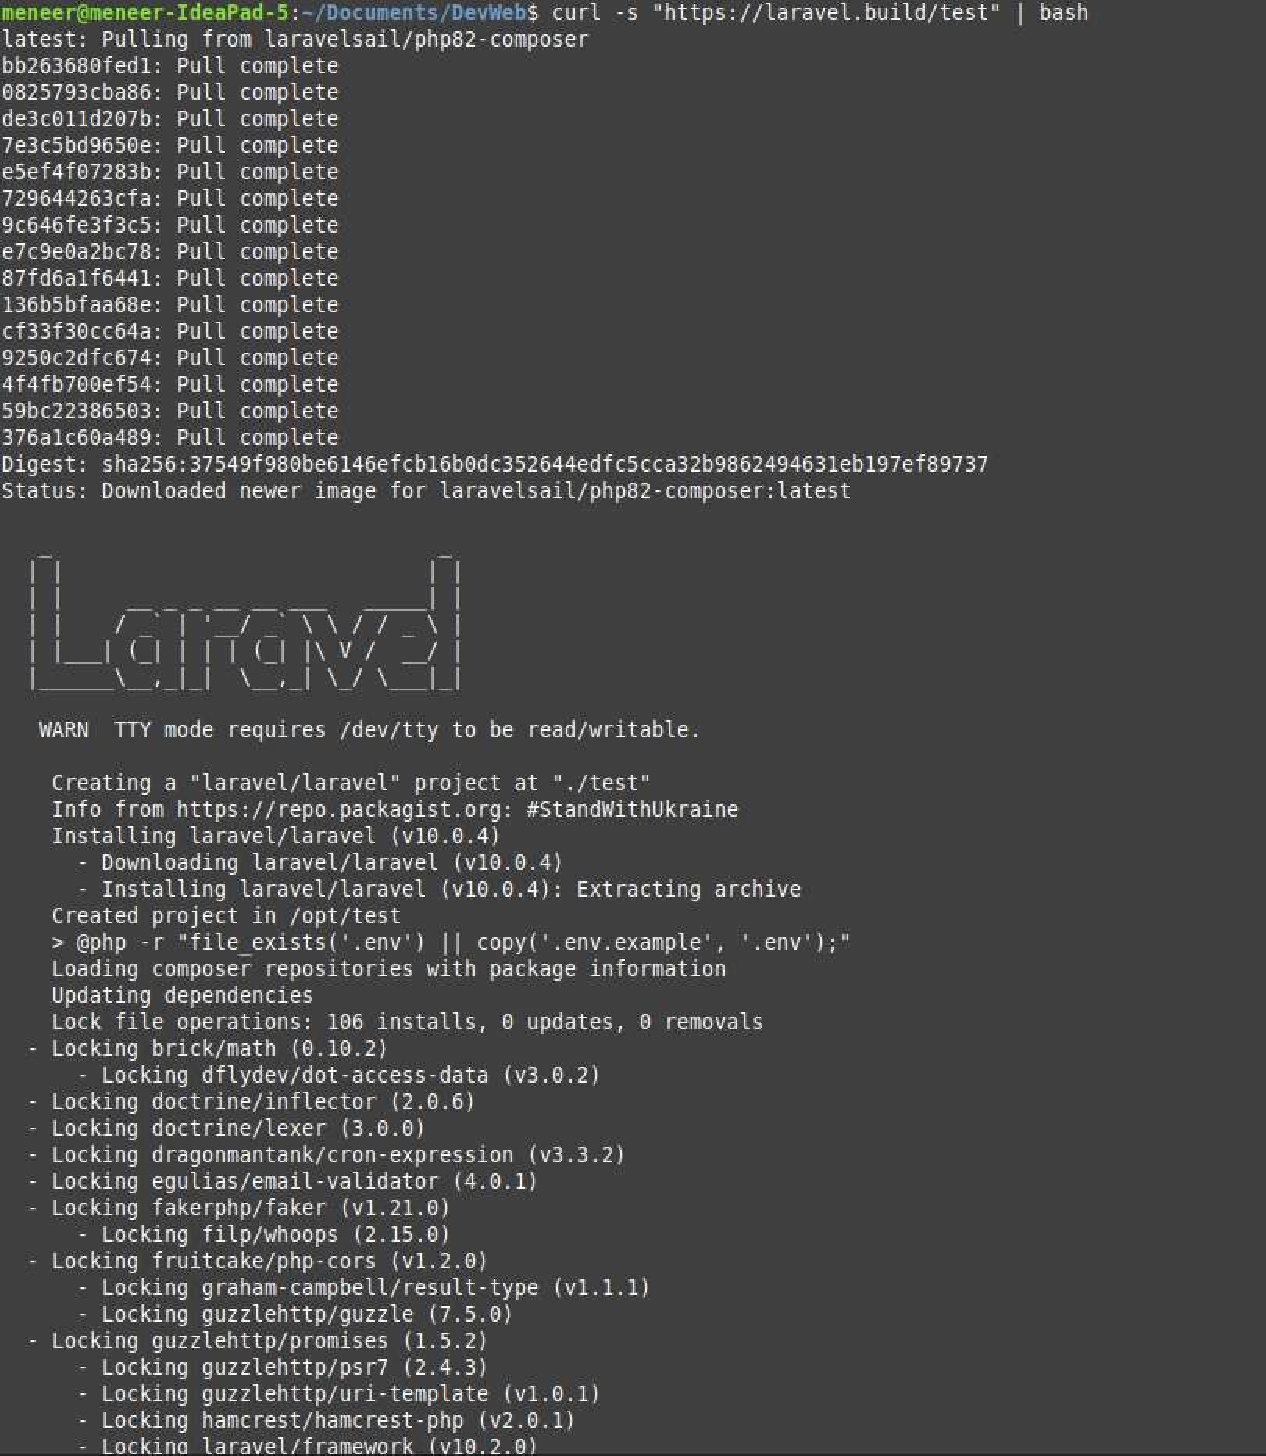
\includegraphics[width=\textwidth]{Images_formation/CreateProject.pdf}
            \end{subfigure}
            \begin{subfigure}{0.3\textwidth}
                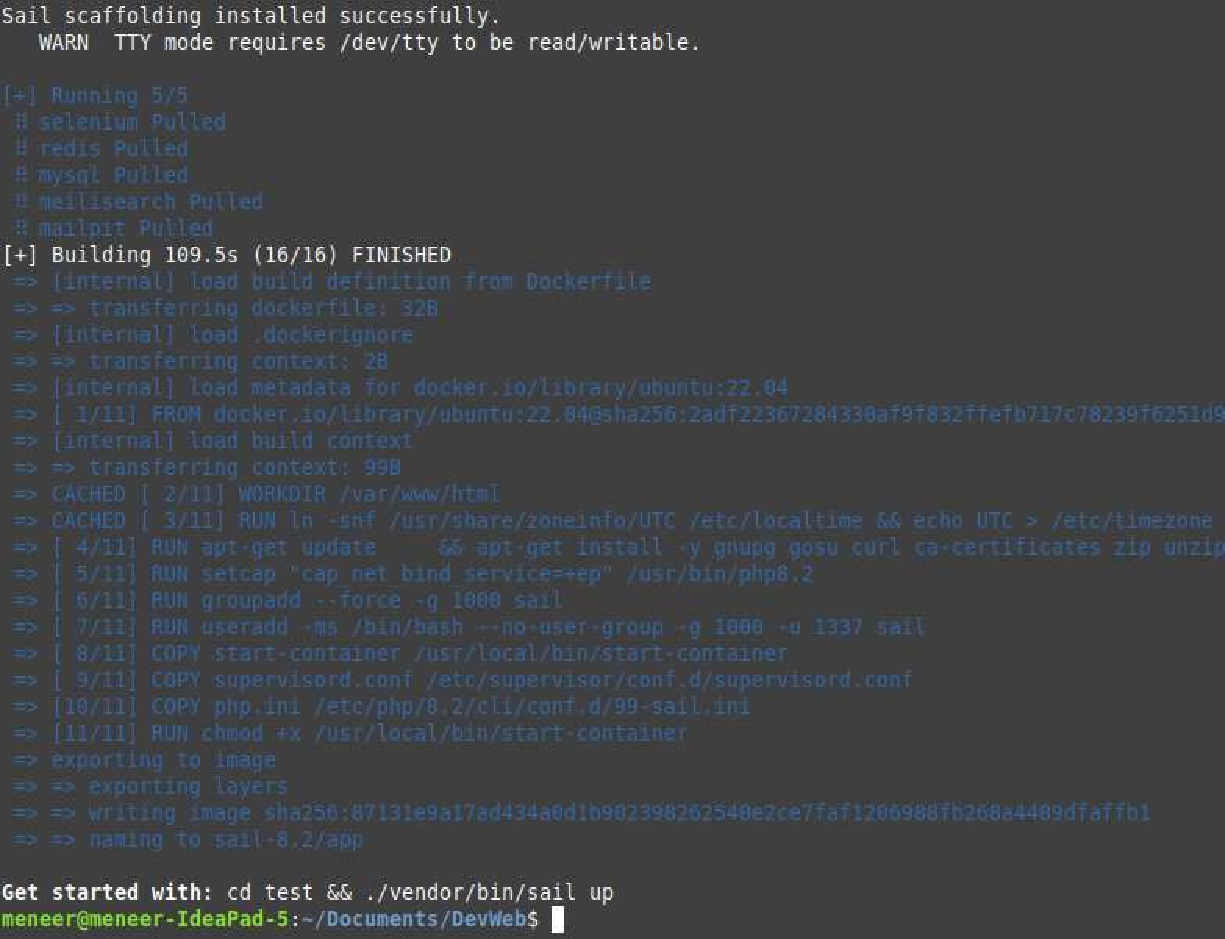
\includegraphics[width=\textwidth]{Images_formation/CreateProject2.pdf}
            \end{subfigure}
        \end{figure}

        Une fois le dossier du projet créé vous allez rentrer dans le dossier (\textit{File} et ensuite \textit{Open Folder\ldots}) et ouvrir le fichier \verb|docker-compose.yml|.

        Ce fichier représente la configuration générale de votre conteneur, c'est ici que l'on va définir les services à installer, les versions, les images, ect.
        Ce fichier est très important, sans lui, pas de conteneur.

        Vous pouvez voir qu'il est composé de plusieurs \href{https://docs.docker.com/compose/compose-file/}{sections}, \textit{Version, services, network, volumes}. Chaque section à son utilitée. Nous allons nous concentrer sur la section \verb|service| du fichier. Plus précisement, nous allons ajouter un service.\\ 


    \subsubsection[Ajout PhpMyAdmin]{Ajout \phpmyadmin{}}

        On va ajouter un service à notre projet qui est nécessaire à la gestion de notre base de donnée,\\ \phpmyadmin{}.
        
        Pour ce faire, rendez-vous à la fin de la section \verb|services|, et ajoutez y \phpmyadmin{} comme suit:

        \begin{lstlisting}
            phpmyadmin:
                image: 'phpmyadmin/phpmyadmin'
                ports:
                    - '8080:80'
                networks:
                    - sail
                environment:
                    - PMA_ARBITRARY=1
                    - PMA_HOST=mysql
                    - PMA_PORT=3306
                depends_on:
                    - mysql
        \end{lstlisting}

        Une fois cela fait, \phpmyadmin{} est intégré au projet.

        \subsubsection{Setup}
        Il y'a plusieurs choses à faire avant de pouvoir accéder à votre site. Premièrement, configurer le fichier \verb|.env|:

        \begin{itemize}
            \item \verb|APP_NAME|: changer le nom de votre application.
            \item \verb|APP_URL|: changer l'URL pour accéder à votre site, attention, cette url doit être conforme à celle écrite dans le fichier \verb|hosts| de la section suivante. Par example, \verb|http://example|.
            \item \verb|DB_DATABASE|: changez le nom de votre \db{} comme bon vous semble.
        \end{itemize}
        Les autres champs peuvent à priori rester inchangés.

        Une fois cela fait, vous pouvez démarer le container avec \verb|sail up -d|.

        Ensuite, installez les librairies \js{} telle que \vite{} avec \verb|sail npm install|

        Enfin, afin de pouvoir accéder à votre site avec l'URL fournie dans le \verb|.env|, il est nécessaire d'ajouter un \textit{localhost}.

        \newpage
        \subsubsection[Localhosts][fr.wikipedia.org/wiki/Localhost]{Localhosts\label{sec:localhost}}
        La méthode diffère selon le système d'exploitation:
        \begin{itemize}
            \item Si vous êtes sous \windows{}, allez dans \verb|C:\Windows\System32\drivers\etc\| et ouvrez le fichier \verb|hosts|\footnote{ATTENTION, vous devez ouvrir ce fichier avec les droits d'administrateur, sinon vous ne pourrez pas sauvegarder vos modifications.}. Dedans, ajoutez deux lignes comme ceci:
            \begin{lstlisting}
                127.0.0.1 example
                ::1 example
            \end{lstlisting}
            \item Si vous êtes sous \linux{}, pareil mais le fichier se trouve dans \verb|/etc/|.
            \item Si vous êtes sous \macos{}, pareil mais le fichier se trouve dans \verb|/private/etc/|.
        \end{itemize}

        Une fois cela fait, redémarez votre navigateur et allez sur l'URL que vous avez choisie, vous devriez voir la page d'acceuil de \laravel{}.

        \hyperref[sec:suite]{Pour passer à la suite}
    
    \newpage
    \subsection[Ajout d'un projet depuis GitHub]{Ajout d'un projet depuis \github{}\label{sec:project_git}}

    Lorsque vous clonez un \texttt{repo} sur votre machine, le site manque des composants essentiels à son fonctionnements: ses packages. Pour installer ces packages, il est nécessaire d'effectuer la commande \verb|composer install|, sauf que vous n'avez pas \texttt{composer} d'installé. En revanche, \texttt{composer} est utilisable grâce à  \laravelsail{} par \verb|sail composer install|!

    Le petit hick, c'est que \laravelsail{} est un package\ldots à installer avec \verb|composer install|\footnote{Le serpent qui se mort la queue, l'oeuf ou la poule, appellez ce paradoxe comme vous le voulez.}. 

    Heureusement, \laravel{} a la sollution pour nous. Il suffit de se rendre dans le dossier de votre projet fraichement installé et de taper:
    \begin{lstlisting}
        docker run --rm \
            -u "$(id -u):$(id -g)" \
            -v "$(pwd):/var/www/html" \
            -w /var/www/html \
            laravelsail/php82-composer:latest \
            composer install --ignore-platform-reqs
    \end{lstlisting}

    de cette manière, les packages de \texttt{composer} seront installés. Plus de renseignements sur la \href{https://laravel.com/docs/10.x/sail#installing-composer-dependencies-for-existing-projects}{Doc \laravel}.
    
    Avec les packages (et donc \laravelsail{}) d'installés, vous pouvez démarer le container avec \verb|sail up -d|.

    En ce qui concerne les librairies \js{}, vous pouvez executer 
    \begin{lstlisting}
        sail npm install
    \end{lstlisting}
    pour installer, entres autres, \vite.

    \subsubsection[Setup]{Setup}
    Enfin, il faut setup les paramètres du site en créant un fichier \verb|.env|\footnote{ps: vous pouvez copier et renommer le fichier \verb|.env example|, mais ne supprimez pas l'original!}. Vous pouvez modifier:

    \begin{itemize}
        \item \verb|APP_NAME|: changer le nom de votre application.
        \item \verb|APP_URL|: changez l'url pour accéder à votre site. Attention, cette url doit être conforme à celle écrite dans le fichier \verb|hosts| de la \textsc{section~\ref{sec:localhost}}
        \item \verb|DB_DATABASE|: changer le nom de votre \db{} comme bon vous semble.
        \item \verb|DB_HOST|: à changer en \verb|mysql|.
    \end{itemize}
    A priori, les autres champs doivent rester inchangés.

    Enfin, il ne vous reste plus qu'à exécuter 
    \begin{lstlisting}
        sail artisan key: generate
    \end{lstlisting}

    et qu'à ajouter l'URL de votre site dans la liste de vos \texttt{localhosts} comme décrit dans la \textsc{section~\ref{sec:localhost}}.

    \subsubsection[Dernières étapes]{Dernières étapes}
    Enfin, les dernière étapes consistent à taper ces deux commandes, que nous expliquerons dans la formation suivante:
    \begin{enumerate}
        \item \verb|sail artisan migrate:fresh --seed| pour lancer la base de donnée.
        \item \verb|sail npm run dev| pour compiler \css{} et \js{}.
    \end{enumerate}

    Une fois cela fait, redémarez votre navigateur et allez sur l'URL que vous avez choisie, vous devriez voir la page d'acceuil de \laravel{}.

    \hyperref[sec:suite]{Pour passer à la suite}
